\documentclass[a4paper]{article}

\usepackage{INTERSPEECH2018}
\usepackage{booktabs}
\usepackage{adjustbox}
\usepackage{multirow}
\usepackage{textcomp}
\usepackage{caption}
\usepackage{subcaption}

\title{Multilingual Multi-Task Learning for Low-Resource Acoustic Modeling}

\name{Josh Meyer}
%The maximum number of authors in the author list is twenty. If the number of contributing authors is more than twenty, they should be listed in a footnote or in acknowledgement section, as appropriate.
\address{
  University of Arizona}
\email{joshua.richard.meyer@gmail.com}

\begin{document}

\maketitle
% 
\begin{abstract}

  The following study investigates low-resource multilingual acoustic model training with Multi-Task Learning (MTL) for Automatic Speech Recognition. The main question of this research is: \textit{What is the best way to represent a source language with MTL to improve performance on the target language?} The two parameters of interest are (1) the level of detail at which the source language is modeled, and (2) the relative weighting of source vs. target languages during backprop.

Results show that when the source task is weighted \textit{higher} than the target task, a \textit{more} detailed task representation (ie. the triphone) leads to better performance on the target language.

On the other hand, when the source task is weighted \textit{lower}, then a \textit{less} detailed level of source task representation (ie. the monophone) is better for performance in the target language. Given all levels of detail in the source task, a 1-to-1 weighting ratio of source-to-target leads to best results on average.

This study uses Kyrgyz (audiobook recordings) as a target language and English (LibriSpeech subset) as a source language.
\end{abstract}

\noindent\textbf{Index Terms}: speech recognition, multi-task learning, acoustic modeling





\section{Introduction}

Performance for a low-resource language on speech recognition can be improved by adding training data from another, resource-rich language. In the Multi-Task Learning (MTL) framework, data from a related source domain updates hidden layers in parallel with the target task \cite{caruana1997}. In ASR, the targets for this addititional language have typically been states of context-dependent triphones, defined by some tree clustering algorithm \cite{huang2013,heigold2013,grezl2016}.

MTL works in situations when tasks are related. For example, the two image recognition tasks (1) find doors and (2) find doorknobs perform better when trained together, because doorknobs are highly predictive of doors, and vice versa \cite{caruana1997}. By forcing a neural net to recognize both objects in the same image, the hidden layers will be biased towards more generalizable representations of the data.

Doors and doorknobs are obviously related, but in general it is difficult to create related tasks for a new classification problem. The current study investigates auxiliary tasks which are not hand-crafted by an expert or human, but can be automatically extracted from a stage in the traditional ASR pipeline (ie. the phonetic decision tree \cite{young1994tree}). The decision tree creates labeled data for the DNN acoustic model, and encodes contextual information about the data. This information is language-specific, and gets more fine-grained further down the tree.

The current research builds off the intuition that the labels created by the decision tree (ie. triphones) encode information which is very specific to the source language, and may not be the best representation of the data for language-transfer. Nodes closer to the roots of the tree represent more abstract levels of the data, and therefore encode more language-general information. Given a phonetic decision tree in a source language (English) the current study investigates more abstract data labels for MTL transfer to a target language (Kyrgyz).

In addition to phonetic detail in the training labels, the relative weighting of the source task vs. target task during backprop affects performance outcomes. If the tasks come from separate datasets, the task with the biggest dataset will have most influence during backprop. To avoid one task dominating the target task, we can weight the training labels for the target task, such that each training example has a larger gradient.

The following experiments show that there is an interaction between task detail and task weighting during MTL. These two factors interact such that, to acheive best results, a more detailed task should be weighted more, and a less detailed task should be weighted less. After an analysis of performance on training and validation data, we see that less detailed (ie. more simple) tasks are easier to learn, and as such, they quickly settle into a good local minumum, and are less likely to budge. However, this local minimum may not be best for the target task.

The target language is Kyrgyz, and the source language is English. Both data come from audiobooks, English from LibriSpeech \cite{panayotov2015} and Kyrgyz from the Bizdin.kg project.




\section{Background}

Past work on MTL for acoustic modeling can be divided into two main categories: monolingual vs. multilingual. Multilingual MTL acoustic modeling involves training a single DNN with multiple output layers, where each output layer represents triphones from one language. Monolingual MTL acoustic modeling involves designing multiple tasks for a single language, where each task is linguistically relevant (eg. triphones vs. monophones vs graphemes).

The earliest examples of MTL with multiple (low-resourced) languages can be found in \cite{huang2013} and \cite{heigold2013}. They were interested in improving performance on all languages, not just one target language. More recently, \cite{grezl2016} studied the effect of adding data from a single, well-resourced language to some low-resourced language.

With regards to monolingual MTL, research has aimed to find tasks (from the same language) which are phonetically relevant to the main task \cite{bell2015}. The aim being to improve generalization to new data. Both \cite{seltzer2013} and later \cite{huang2015} looked at a very similar approach, definig additional auxiliary tasks in MTL via broad, abstract phonetic categories for English. With regards to low-resource languages, \cite{chen2014} and later \cite{chen2015} similarly looked at MTL for a single target language, using graphemes or a universal phoneset as extra targets.



\section{DNN-Hybrid Training as Model Transfer}

The standard DNN-Hybrid approach uses an initial GMM-HMM system to generate the labeled data for supervised DNN training. This reliance of the DNN on GMM alignments is actually a form of model transfer, where the DNN is trained to perform the extact same classification as its GMM predecessor. The DNN not only learns the frame alignments from the individual GMMs, but also the structure of the phonetic decision tree used to define the labels, as shown in Figure (\ref{fig:tree-net})\footnote{The original decision tree graphic comes from \cite{young2002}, and the original neural net graphic comes from \cite{heigold2013}}.


\begin{figure}[!htbp]
  \centering
\minipage{0.5\textwidth}
  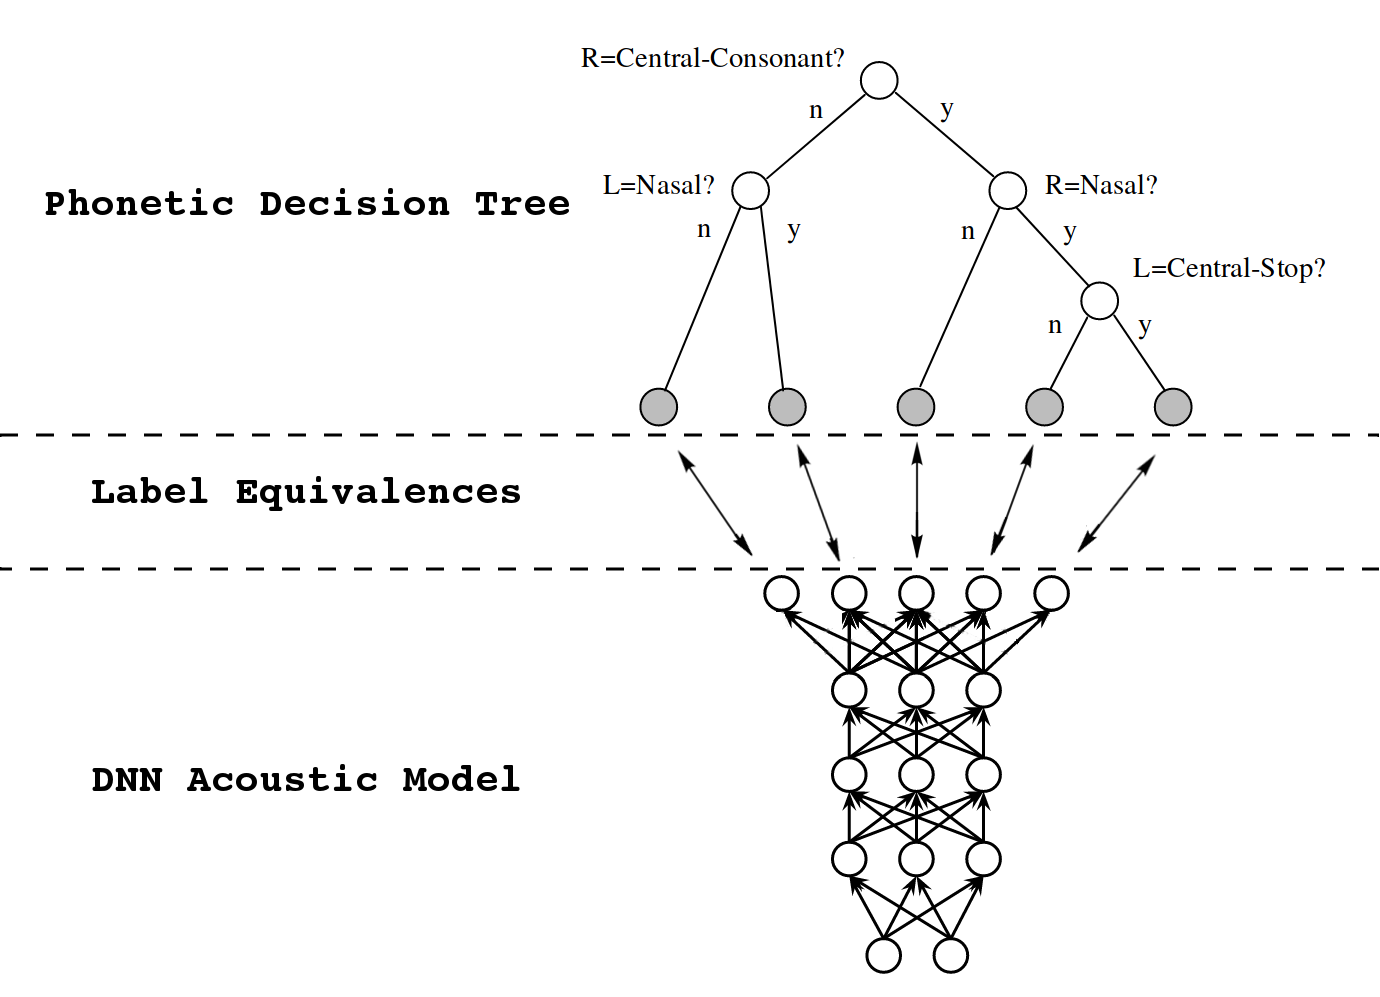
\includegraphics[width=\linewidth]{figs-1/tree-net.png}
  \caption{GMM$\rightarrow$DNN Model Transfer}
    \label{fig:tree-net}
  \endminipage\hfill
\end{figure}

However, all heirarchical knowledge inherent to the decision tree is lost to the DNN. The DNN only sees the leaves of the tree, but none of the relationships among those leaves. The branches and roots are lost, which contain more abstract, language-general knowledge. The current study extracts the heirarchical knowledge of this tree via MTL, by modeling various levels of the tree as separate tasks. 


\section{Experiments}

The following experiments tease out (1) the level of detail at which the source language should be modeled and (2) the amount of weighting which should be given to the target language training examples.

With regards to the first point, the experiments here are crafted to answer the question: \textit{How much phonetic detail should the source language be modeled at to best transfer inductive bias to the target language?}

We can model the source language with lots of contextual detail (ie. the triphone), with abstracted, context-independent detail (ie. the monophone), or somewhere in between (what I dub the ``half''-phone) (cf. Figure (\ref{fig:tree-parts})\footnote{Original figure from \cite{young2002}.}).


\begin{figure}[!htbp]
  \centering
\minipage{0.525\textwidth}
  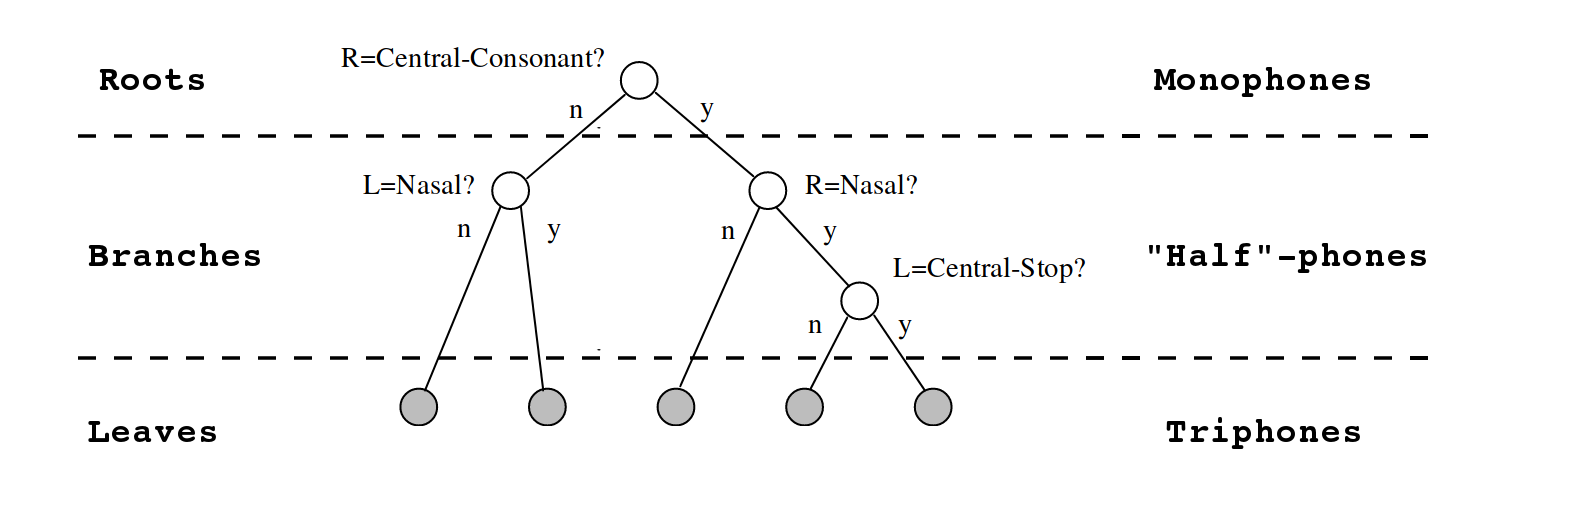
\includegraphics[width=\linewidth]{figs-1/levels.png}
  \caption{Logical Tree Parts}
  \label{fig:tree-parts}
\endminipage\hfill
\end{figure}



The second point of interest is the relative weighting of target vs. source language training data. It is clear that if we train two languages in parallel, the source language (with many more training samples) will dominate the target language in the fight for influence over shared hidden layers during backprop.

To my knowledge, the importance of relative weighting has not been investigated in ASR acoustic modeling (although it was dedicated its own chapter in Caruana's 1997 dissertation \cite{caruana1997}). To investigate weighting further, I examine the following weighting schemes: 1-to-2, 1-to-1, and 2-to-1 (all ratios are source-to-target).

These weights are instantiated during training via a weight to the target output label, where the label is a one-hot vector. For example, given 1000 hours of source language and 1 hour of target language, to acheive a 1-to-1 ratio in training, I would multiply the target labels from the target language by 1000, resulting in target vectors such as \texttt{$[0, 0, 0, 0, 1000, 0, 0, \ldots]$} instead of \texttt{$[0, 0, 0, 0, 1, 0, 0, \ldots]$}.



\subsection{Data}

Two speech corpora are used in the following experiments:

\begin{enumerate}
\item $\approx$ 5 hours of English (4.86 hours of LibriSpeech)
\item $\approx$ 1.5 hours of Kyrgyz (1.59 hours of audiobook)
\end{enumerate}

\subsection{Model Building}

All models were build using the Kaldi toolkit as Time-Delay Neural Networks (TDNNs) via the \texttt{nnet3} approach \cite{povey2011,peddinti2015}. The main neural net run script used in this paper can be found at www.github.com/JRMeyer/kaldi-mirror/egs/kgz/kyrgyz-model/run\_nnet3\_multilingual.sh. The main GMM script used to create data alignments can be found at www.github.com/JRMeyer/kaldi-mirror/egs/kgz/kyrgyz-model/run\_gmm.sh.

In GMM training, monophones (for each language) were allotted 1,000 Gaussian components, and trained over 25 iterations of EM. These monophones were then expanded into context-dependent triphones via a phonetic decision tree, with a maximum of 2,000 leaves \& 5,000 Gaussians (LibriSpeech reached 1584 leaves, and Kyrgyz reached 752). The resulting tied-state clusters (ie. leaves) are then trained as context-dedendent triphones over 25 iterations of EM.

Given the alignments from the GMM-HMM models, a 5-layer, 500-dimensional TDNN is trained over 10 epochs of backprop on a single GPU instance.

Each auxiliary task is implemented as a separate output layer along with a separate, penultimate hidden layer. All other hidden layers of the TDNN are trained in parallel. A declining learning rate was used, with an initial $\alpha_{initial}=0.0015$ and a final $\alpha_{final}=0.00015$. The objective function is $max( KaldiBatchNorm(ReLU\_activation) \bullet target )$.

During testing, \textit{only} the main task is used. The additional tasks are dropped and the baseline Kyrgyz triphones are used in decoding. This highlights the purpose of the extra tasks: to force the learning of robust representations in the hidden layers during training; they serve as ``training wheels'' which are then removed once the net is ready.



\subsubsection{Baseline Model}

All the following architectures will be compared to the performance of a baseline model of identical architecture (5 hidden layers, 500-dimentional layers, ReLU activations, same linear objective function). The output targets are standard context-dependent triphones trained on Kyrgyz audio.

To account for any advantage mutliple output layers may bring about, the baseline contains two output layers, where the tasks are identical. In this way, random initializations in the weights and biases for each task are accounted for.

\subsubsection{Auxiliary Tasks}

The auxiliary tasks all train on English language data from the LibriSpeech corpus. Investigating the intuition that labels generated by a standard triphone phonetic decision tree are not the best representation of data for transfer learning, the auxiliary tasks here investigate different levels in the decision tree's branches.

I split the LibriSpeech phonetic decision tree into three logical parts, shown in Figure (\ref{fig:tree-parts}):

\begin{enumerate}
\item roots (standard monophones)
\item branches (custom ``half''-phones)
\item leaves (standard triphones)
\end{enumerate}



The ``half''-phones were created by halving the optimal number of leaves from the triphone system (ie. 1584 leaves) and re-training a new GMM-HMM system with half the optimal number of leaves (1/2 * 1584 = 792 leaves). All the other parameters were left unchanged (number of Gaussian components, iterations of EM, etc.). An overview of the auxiliary tasks can be found in Table (\ref{tab:tasks}).




\begin{table}[!htbp]
  \centering
  \caption{Auxiliary Tasks}
  \label{tab:tasks}
  \begin{adjustbox}{width=.45\textwidth}
    \begin{tabular}{lcc}
      \toprule
      \textbf{Logical Tree Part} & \textbf{Level of Phonetic Detail} & \textbf{ \textnumero~of Tasks}\\
      \midrule
      Roots & Monophones & 1\\
      Branches & Half-phones & 1\\
      Leaves & Triphones & 1\\ 
      Lower Tree & Monophones + Half-phones & 2\\
      Upper Tree & Half-phones + Triphones & 2\\
      Whole Tree & Monophones + Half-phones + Triphones & 3\\
      \bottomrule
    \end{tabular}
  \end{adjustbox}
\end{table}

By forcing the neural net to recognize higher levels in the English source tree, we will learn representations which are more abstract, and therefore more likely to be relevant multi-lingually. 


\subsubsection{Weighting Procedure}

The addition of each above task adds approximately 5 hours of training data to the standard training of a Single Task Model on Kyrgyz. As such, a weighting procedure was used to balance the relative influence of source vs. target training data on backprop. For example, to reach a one-to-one ratio, where one hour of Kyrgyz is equal to one hour of English, I multiplied every Kyrgyz target one-hot vector by $3.06$. The exact weighting scheme is shown in Table (\ref{tab:weights}).

\begin{table}[!htbp]
  \centering
  \caption{Source:Target Data Weighting Scheme}
  \label{tab:weights}
  \begin{adjustbox}{width=.33\textwidth}
    \begin{tabular}{cc}
      \toprule
      \textbf{Source:Target Ratio} & \textbf{Target Weighting}\\
      \midrule
      2:1 & 1.53x  \\
      1:1 & 3.06x  \\
      1:2 & 6.12x  \\
      \bottomrule
    \end{tabular}
  \end{adjustbox}
\end{table}




\subsection{Results}


All results come from performance on the same held-out 30-minute section of Kyrgyz audiobook. Decoding is performed with a bigram backoff language model trained on a Wikipedia Kyrgyz dump, and contains, 103,998 unigrams and 56,6871 bigrams. The bigram language model, lexicon, and main-task decision tree are built into a standard decoding graph (ie. a Weighted Finite State Transducer) in the traditional Kaldi pipeline. 

The experimental results are shown in Table (\ref{tab:results}) as percent Word Error Rate (WER) relative to the baseline model. All experiments show improvement over the baseline. Each column has in bold the model which performed best (the bottom row has also the bolded best average weighting).

\begin{table}[!htbp]
  \centering
  \caption{Word Error Rates (WER\%) Relative to Baseline}
    \label{tab:results}
  \begin{adjustbox}{width=.475\textwidth}
    \begin{tabular}{lcccc}
      \toprule
      & \multicolumn{4}{c}{\textbf{Source:Target Weighting}} \\
      \textbf{Auxiliary (Source Lang) Tasks} & \textit{1-to-2} & \textit{1-to-1} & \textit{2-to-1} & AVERAGE\\
      \midrule
      STL Baseline                          &               \multicolumn{4}{c}{50.54\% WER}  \\
      Monophones                            & \textbf{-2.34}  & -3.22           & -3.13           & \textbf{-2.90}\\
      Halfphones                            & -1.86           & \textbf{-3.81}  & -1.86           & -2.51\\
      Triphones                             & -1.17           & -3.42           & \textbf{-3.81}  & -2.80\\
      Monophones + Halfphones               & \textbf{-2.34}  & -2.05           & -2.44           & -2.28\\
      Halfphones + Triphones                & -0.49           & -2.54           & -2.64           & -1.89\\
      Monophones + Halfphones + Halfphones  & -1.66           & -2.34           & -1.95           & -1.98\\
      \midrule
      AVERAGE                               & -1.64           & \textbf{-2.90}  & -2.64           & \\
      \bottomrule
    \end{tabular}
  \end{adjustbox}
\end{table}

We see that on average, across all tasks and task combinations, a 1-to-1 weighting performed the best with an average 2.90\% improvement over the baseline. Averaged over all weighting schemes, the best auxiliary task was English monophones (most abstract task).

The best overall combination of weighting and source task detail was a tie between (1) triphones + 2-to-1 weighting and (2) half-phones + 1-to-1 weighting. Even though on average the abstract source task labels (monophones) performed better, the more detailed source tasks acheived best WER in a single run (3.81\% improvement).

Comparing performance among combinations of auxiliary tasks, we see that MTL training with just one auxiliary task always performed better than two or three extra source tasks.



%% \begin{table}[!htbp]
%%   \centering
%%     \caption{TDNN // 5-layer // 500-dim //  10 epoch }
%%   \begin{adjustbox}{width=.45\textwidth}
%%     \begin{tabular}{lccc}
%%       \toprule
%%       & \multicolumn{3}{c}{\textbf{Target:Source Weighting}} \\
%%       \textbf{Auxiliary (Source Lang) Tasks} & \textit{1-to-2} & \textit{1-to-1} & \textit{2-to-1}\\
%%       \midrule
%%       STL Baseline                          &  \multicolumn{3}{c}{50.54}  \\
%%       Monophones                            &  47.41  & 47.32 & 48.20  \\
%%       Halfphones                            &  48.68  & 46.73 & 48.68 \\
%%       Triphones                             &  46.73  & 47.12 & 49.37  \\
%%       Monophones + Halfphones               &  48.10  & 48.49 & 48.20 \\
%%       Halfphones + Triphones                &  47.90  & 48.00 & 50.05\\
%%       Monophones + Halfphones + Halfphones  &  48.59  & 48.20 & 48.88\\
%%       \bottomrule
%%     \end{tabular}
%%     \label{table:data}
%%   \end{adjustbox}
%% \end{table}





\begin{figure*}[!htbp]
\centering
\begin{subfigure}{.33\textwidth}
  \centering
  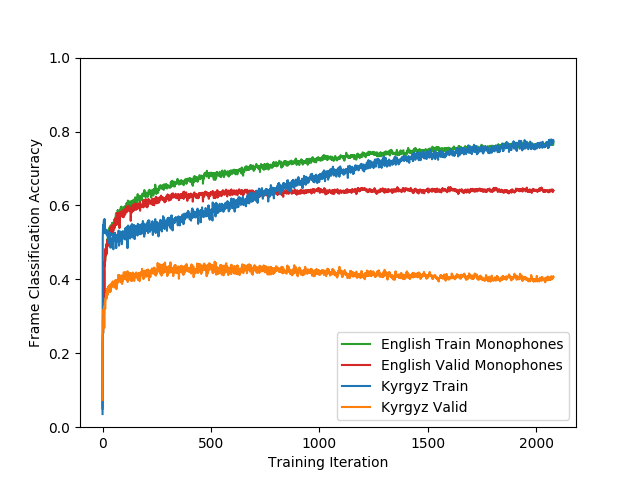
\includegraphics[width=1\textwidth,keepaspectratio]{figs-1/2-to-1-mono.png}
  \caption{1-to-2 Weighting // Monophones}
  \label{fig:sub1}
\end{subfigure}%
\begin{subfigure}{.33\textwidth}
  \centering
  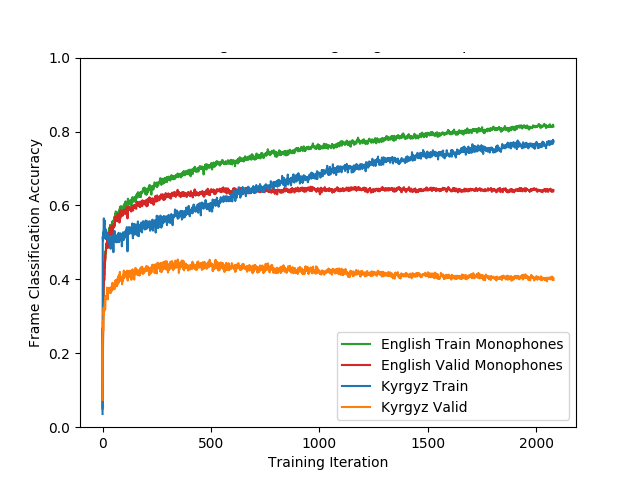
\includegraphics[width=1\textwidth,keepaspectratio]{figs-1/1-to-1-mono.png}
  \caption{1-to-1 Weighting // Monophones}
  \label{fig:sub2}
\end{subfigure}%
\begin{subfigure}{.33\textwidth}
  \centering
  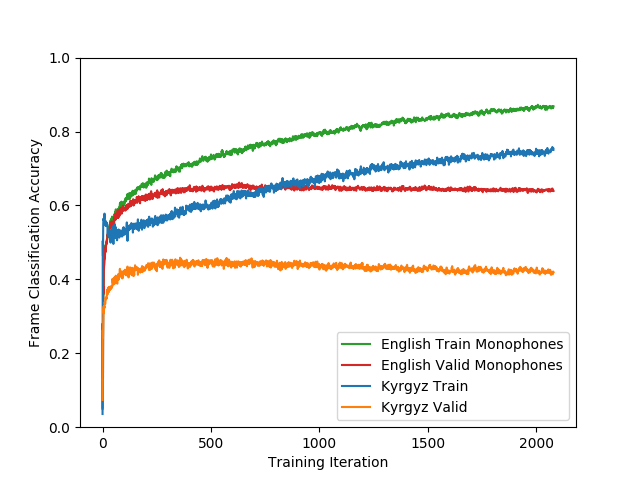
\includegraphics[width=1\textwidth,keepaspectratio]{figs-1/1-to-2-mono.png}
  \caption{2-to-1 Weighting // Monophones}
  \label{fig:sub2}
\end{subfigure}

\medskip

\begin{subfigure}{.33\textwidth}
  \centering
  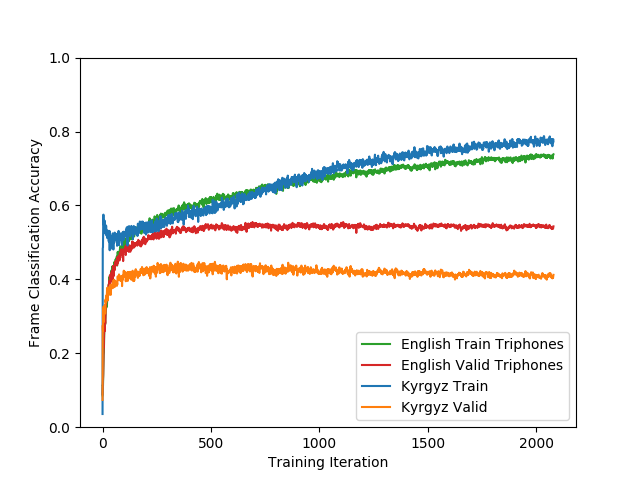
\includegraphics[width=1\textwidth,keepaspectratio]{figs-1/2-to-1-tri.png}
  \caption{1-to-2 Weighting // Triphones}
  \label{fig:sub1}
\end{subfigure}%
\begin{subfigure}{.33\textwidth}
  \centering
  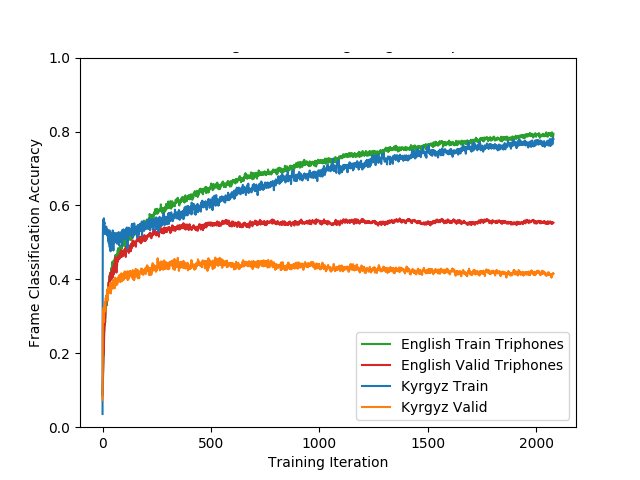
\includegraphics[width=1\textwidth,keepaspectratio]{figs-1/1-to-1-tri.png}
  \caption{1-to-1 Weighting // Triphones}
  \label{fig:sub2}
\end{subfigure}%
\begin{subfigure}{.33\textwidth}
  \centering
  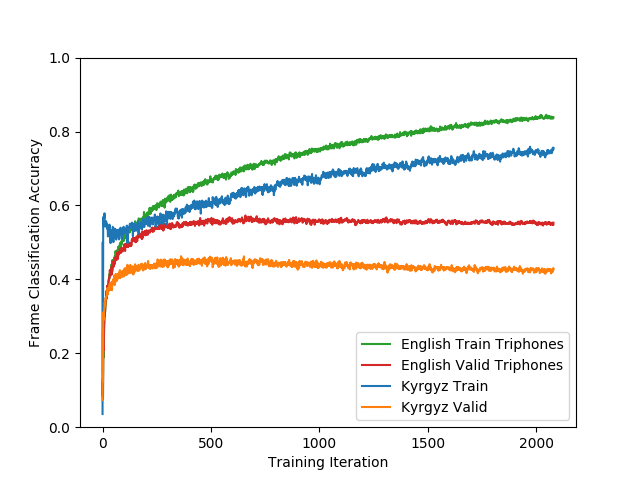
\includegraphics[width=1\textwidth,keepaspectratio]{figs-1/1-to-2-tri.png}
  \caption{2-to-1 Weighting // Triphones}
  \label{fig:sub2}
\end{subfigure}
\caption{Source:Target Weighting vs. Source Task Detail}
\label{fig:1-to-2}
\end{figure*}



\section{Discussion}

Perhaps the most interesting finding is the interaction between level of detail in individual source tasks and relative weighting during training. We find that in general, the less detail in the source task, the less weight we should give it during training. The monophones were the exception to the rule, getting best performance with 1-to-1 weighting. The following discussion will focus on this interaction (ie. experiments represented in the first three columns of Table (\ref{tab:results})). 

A task with fewer labels is typically easier to learn, finds a local minimum more quickly, and is less willing to budge once it is settled. A more difficult source task will take longer to learn, and as such, the target task will be able to exert more influence on the shared hidden layers.

Figure (\ref{fig:1-to-2}) shows performance (ie. frame-level classification accuracy) during training with one of two auxiliary tasks (cf. Figure(\ref{fig:1-to-2}) rows) and three weighting schemes (cf. Figure(\ref{fig:1-to-2}) columns). The source task is weighted heavier in the left column, and in the right column the target task is weighted more. The top row shows experiments with English monophones as source task, and the bottom row shows English triphones as a source task. The Green vs Blue lines represent training data accuracy (for English vs. Kyrgyz respectively). The Red vs. Orange lines represent validation data accuracy (for. English vs. Kyrgyz respectively).

We see most overfitting to the target data in Figure (\ref{fig:1-to-2}d), where the source task is most detailed (triphones), and the source data is only weighted half as much as the target data during training. This model performed substantially worse than all others shown here, with only a 1.17\% WER improvement over baseline.

Looking up to Figure (\ref{fig:1-to-2}c) we see the other extreme, where the source task is weighted twice as much as the target task, and the source task is very simple (monophones). The gap between tasks is widest in this setting, because the source task finds a good local minimum quickly, and the target data never has enough weight to influence the hidden layers.

These results indicate that merely adding related tasks in training via MTL is not enough to guarantee optimal transfer - one must consider task difficulty and weight accordingly. 




\section{Conclusions}

Multi-Task Learning promises a very simple solution to a very hard problem. It would seem that as long as we can add relevant tasks to our net, through the good graces of backprop, a best solution will automatically be discovered. It would also seem that we are guaranteed to get better results as long as we keep adding related tasks. This study shows that the picture is not so simple.

Starting with three additional tasks, which are clearly related \textit{a priori}, the current study investigated not only their relative import, but also the dynamics of their combinations. Each task represents a level of abstraction from the typical training labels, from fine-grained (triphones), to more abstract (half-phones) to completely context-free (monophones). In addition to these three levels (deduced from a given decision tree), I tested logical combinations of abstractions: the entire tree, the top half of the tree, and the bottom half of the tree. None of these combinations outperformed the tasks added individually.

The interaction of differential task weighting and level of task detail was perhaps the most interesting finding of the current study. The level of task abstraction correlates to number of labels in the task, number of nodes in the output layer, and number of parameters in the model.

With more labels, the task is inherently more difficult and the model has more parameters to train. As such, models with fewer labels found their local minimum more quickly, and were more likely to exert influence over shared hidden layers than some other task (ie. Kyrgyz).

In similar MTL setups, care should be taken to weighting auxiliary tasks relative to their simplicity, even if tasks are related.



\section{Acknowledgements}

I'd like to thank Dan Povey for answering my (oftentimes naive) questions on the kaldi-help Google Group.

I'd like to also thank Chorobek Saadanbekov and Murat Jumashev for making the Kyrgyz audiobook available to me through the Bizdin.kg group.

This material is based upon work supported by the National Science Foundation Graduate Research Fellowship under Grant No. (DGE-1746060). Any opinion, findings, and conclusions or recommendations expressed in this material are those of the authors(s) and do not necessarily reflect the views of the National Science Foundation.





\newpage

\bibliographystyle{IEEEtran}
\bibliography{mybib}



\end{document}
